\documentclass{beamer}
\usepackage{amssymb}
\usepackage{subcaption}
\usepackage{natbib}
\usepackage{tikz}
\usepackage{pdfpcnotes}
\usepackage{tikz-qtree}
\usepackage{mathtools}
\usepackage{textpos}
\usepackage{stackengine} 
\newcommand\oast{\stackMath\mathbin{\stackinset{c}{0ex}{c}{0ex}{\ast}{\bigcirc}}}
%\usepackage{pifont}
\newcommand{\smallspace}{\hspace{1mm}}
% \definecolor{macolor}{rgb}{1.0, 0.3, 0.1}
% \setbeamercolor{alerted text}{fg=macolor}

\graphicspath{{./images/}}
\mode<presentation> {
\usetheme{Madrid}

% \usecolortheme{albatross}
% \usecolortheme{beaver}
% \usecolortheme{beetle}
% \usecolortheme{crane}
% \usecolortheme{dolphin}
% \usecolortheme{dove}
% \usecolortheme{fly}
% \usecolortheme{lily}
% \usecolortheme{orchid}
% \usecolortheme{rose}
% \usecolortheme{seagull}
% \usecolortheme{seahorse}
% \usecolortheme{whale}
% \usecolortheme{wolverine}

% \setbeamertemplate{footline} % To remove the footer line in all slides uncomment this line
\setbeamertemplate{footline}[page number] % To replace the footer line in all slides with a simple slide count uncomment this line

\setbeamertemplate{navigation symbols}{} % To remove the navigation symbols from the bottom of all slides uncomment this line
}

%\usepackage{graphicx} % Allows including images
\usepackage{booktabs} % Allows the use of \toprule, \midrule and \bottomrule in tables

%%----------------------------------------------------------------------------------------
%%	TITLE PAGE
%%----------------------------------------------------------------------------------------

\title[RL of Theorem Proving]{Reinforcement Learning of Theorem Proving} % The short title appears at the bottom of every slide, the full title is only on the title page

%\author{Dobrik Georgiev} % Your name
%\institute[Cambridge] % Your institution as it will appear on the bottom of every slide, may be shorthand to save space
%{
%\textit{dgg30@cam.ac.uk.com} % Your email address
%}
\date{} % Date, can be changed to a custom date
\author{{\footnotesize a paper by}\\\textit{Cezary Kaliszyk, Josef Urban,
Henryk Michalewski and Miroslav Ol\v{s}{\'{a}}k}\\~\\{\footnotesize
presented by}\\\textit{Dobrik Georgiev}}

\AtBeginSection[]
{
  \begin{frame}<beamer>
    % \frametitle{Outline for section \thesection}
    \tableofcontents[currentsection]
  \end{frame}
}

\begin{document}

\begin{frame}
\titlepage % Print the title page as the first slide
\end{frame}

\begin{frame}
\frametitle{Overview} % Table of contents slide, comment this block out to remove it
\tableofcontents % Throughout your presentation, if you choose to use \section{} and \subsection{} commands, these will automatically be printed on this slide as an overview of your presentation
\end{frame}
\section{How tableau provers work} 

\begin{frame}
    \frametitle{How tableau provers work}
    \only<1-1>{
    \begin{columns}
        \column{.45\textwidth}
        \small
        Clauses:
        \begin{itemize}
            \item[$c_1$]: $P(X)$
            \item[$c_2$]: $R(X, Y) \lor \neg P(X) \lor Q(Y)$
            \item[$c_3$]: $S(X)\lor \neg Q(b)$
            \item[$c_4$]: $\neg S(X)\lor \neg Q(X)$
            \item[$c_5$]: $\neg Q(X)\lor \neg R(a, X)$
            \item[$c_6$]: $\neg R(a, X)\lor Q(X)$
        \end{itemize}
        % \pause
        \column{.60\textwidth}
            \centering
            \begin{figure}
            \caption{A closed tableau}
            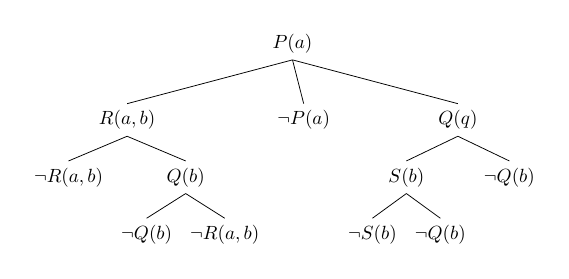
\begin{tikzpicture}[scale=0.69]
            \tikzset{level 1/.style={level distance=40pt}}
            % \tikzset{level 2/.style={level distance=40pt}}
            % \tikzset{level 3/.style={level distance=40pt}}
            % \tikzset{edge from parent/.append style{very thick}}
            \tikzset{sibling distance=1mm}
            \Tree
            [.$P(a)$
                [.$R(a,b)$
                    [.$\neg R(a,b)$ ]
                    [.$Q(b)$
                        [.$\neg Q(b)$ ]
                        [.$\neg R(a,b)$ ]
                    ]
                ] 
                [.$\neg P(a)$ ] 
                [.$Q(q)$
                    [.$S(b)$
                        [.$\neg S(b)$ ]
                        [.$\neg Q(b)$ ]
                    ]
                    [.$\neg Q(b)$ ]
                ] 
            ]
            \end{tikzpicture}
            \end{figure}
    \end{columns}
    }
    % \only<3>{
    %     \begin{figure}
    %     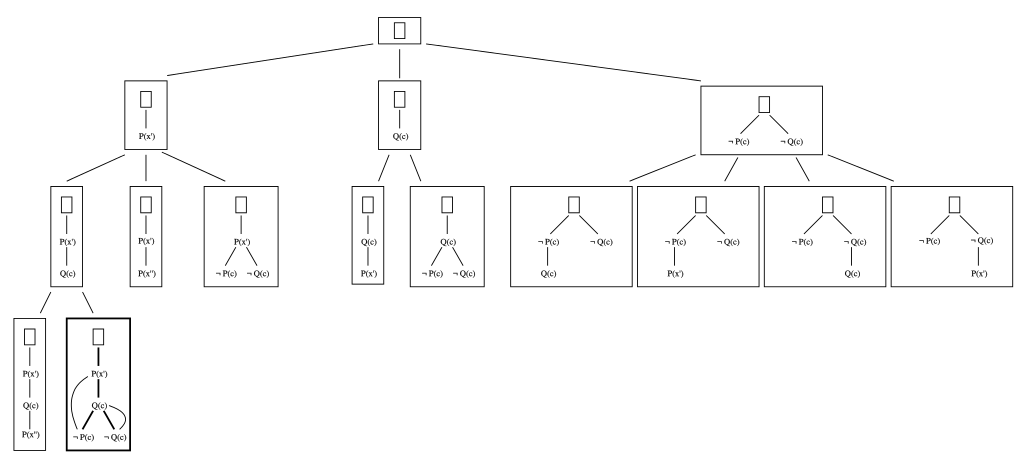
\includegraphics[width=\linewidth]{tableaux.png}
    %     \caption{The search tree of a (non-connection) tableau based TP}
    %     \end{figure}
    % }

    % \begin{figure}
    % 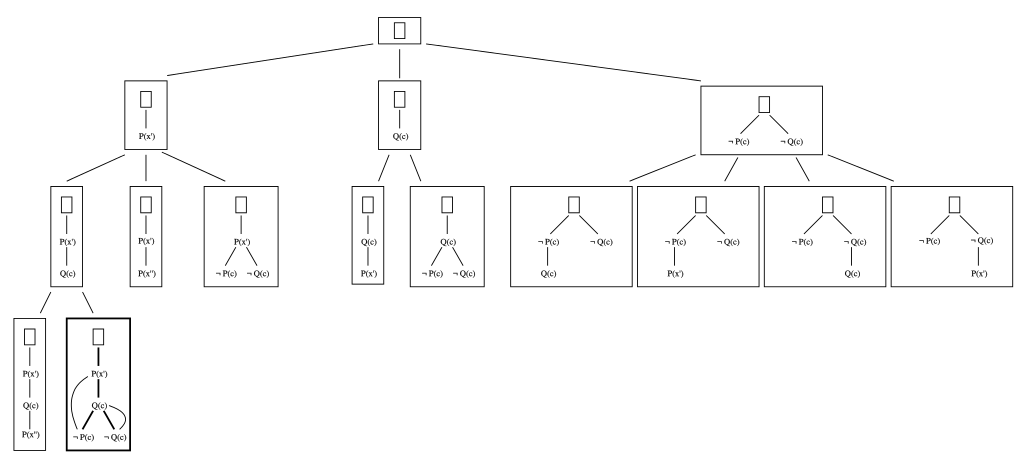
\includegraphics[width=\linewidth]{tableaux.png}
    % \caption{The search tree of a tableau based TP\footnote{Source: Wikipedia}}
    % \end{figure}

\end{frame}
% \begin{frame}
%     \frametitle{Connection Tableau - how it works}
%     Assume the classical proof by contradiction setting
%     \begin{itemize}
%         \item Translate the formula to CNF
%         \item Skolemize
%         \item Represent as set of clauses
%         \item Proof proceeds by building tableau with \alert{connections}
%             \begin{itemize}
%                 \item ($L$, $\neg{L}$) is a \alert{connection}
%                 \item We will see an example
%             \end{itemize}
%         \item Successful proof $\iff$ connection in every path from root to leaf
%     \end{itemize}
% \end{frame}

% \begin{frame}
%     \frametitle{Connection Tableau - an example}
%     \begin{columns}
%         \column{.45\textwidth}
%         Consider\footnotemark:
%         \begin{align*}
%             &\begin{aligned}
%                 \{P,\smallspace R\} \smallspace
%                 \{\neg{P},\smallspace X \}\smallspace
%                 \{\neg{b},\smallspace P\}\smallspace
%             \end{aligned}\\
%             &\begin{aligned}
%                 \{\neg{c },\smallspace \neg{P}\}\smallspace
%                 \{P,\smallspace \neg{R}\}
%             \end{aligned}
%         \end{align*}

%         \begin{itemize}
%             \item<2-> Start rule
%             \item<3-> Extension rule
%             \item<5-> Reduction rule
%         \end{itemize}
%         \column{.45\textwidth}
%                 \centering
%                 \only<2>{
%                     \begin{tikzpicture}[remember picture, overlay]
%                     \tikzstyle{level 1} = [level distance=.8cm, sibling distance=30mm]
%                     \tikzstyle{level 2} = [level distance=1cm, sibling distance=10mm]
%                     \tikzstyle{level 3} = [level distance=1cm, sibling distance=10mm]
%                     % \tikzset{every tree node/.style={anchor=center, scale=0.84}}
%                     \node (s) at (0, 2) {}
%                         child { node{$P$} }
%                         child { node{$R$} };
%                     \end{tikzpicture}%
%                 }%
%                 \only<3>{
%                     \begin{tikzpicture}[remember picture, overlay]
%                     \tikzstyle{level 1} = [level distance=.8cm, sibling distance=30mm]
%                     \tikzstyle{level 2} = [level distance=1cm, sibling distance=10mm]
%                     \tikzstyle{level 3} = [level distance=1cm, sibling distance=10mm]
%                     % \tikzset{every tree node/.style={anchor=center, scale=0.84}}
%                     \node (s) at (0, 2) {}
%                         child { node{$P$}
%                             child { node{$\neg{P}$} }
%                             child { node{$X'$} } }
%                         child { node{$R$} };
%                     \end{tikzpicture}%
%                 }%
%                 \only<4-5>{
%                     \begin{tikzpicture}[remember picture, overlay]
%                     \tikzstyle{level 1} = [level distance=.8cm, sibling distance=30mm]
%                     \tikzstyle{level 2} = [level distance=1cm, sibling distance=10mm]
%                     \tikzstyle{level 3} = [level distance=1cm, sibling distance=10mm]
%                     % \tikzset{every tree node/.style={anchor=center, scale=0.84}}
%                     \node (s) at (0, 2) {}
%                         child { node (p) {$P$}
%                             child { node {$\neg{P}$} }
%                             child { node{$X'$}
%                                 child{ node{$\neg{c}$} }
%                             child{ node (negp) {$\neg{P}$} } } }
%                         child { node{$R$} };
%                     \only<5>{\draw[densely dashed] (p) to [bend left=50,auto] (negp);}
%                     \end{tikzpicture}%
%                 }%
%                 \only<6>{
%                     \begin{tikzpicture}[remember picture, overlay]
%                     \tikzstyle{level 1} = [level distance=.8cm, sibling distance=30mm]
%                     \tikzstyle{level 2} = [level distance=1cm, sibling distance=10mm]
%                     \tikzstyle{level 3} = [level distance=1cm, sibling distance=10mm]
%                     % \tikzset{every tree node/.style={anchor=center, scale=0.84}}
%                     \node (s) at (0, 2) {}
%                         child { node{$P$}
%                             child { node{$\neg{P}$} }
%                             child { node{$X'$}
%                                 child{ node{$\neg{c}$} }
%                                 child{ node{$\neg{P}$} } } }
%                         child { node{$R$}
%                             child { node{$P$}
%                                 child { node{$\neg{P}$} }
%                                 child { node{$X''$}
%                                     child{ node{$\neg{c}$ } }
%                                     child{ node{$\neg{P}$ } }
%                                 }
%                             }
%                             child { node{$\neg{R}$} } };
%                     \end{tikzpicture}%
%                 }%
%     \end{columns}
%     \footnotetext[1]{Example adapted from\\ \url{http://www.leancop.de/atp-fub12/atp_fub12_3cop.pdf}}
% \end{frame}
% \subsection{Semantics of Connection Tableau}

% \subsection{Searching for a Closed Tableau}

\section{Reinforcement Learning and Application to TP}

\begin{frame}
    \frametitle{RL Basics}
    \begin{columns}
    \column{.7\textwidth}
    \begin{figure}
        \begin{tikzpicture}
            \node[anchor=south, inner sep=0] (image) at (0, 0) {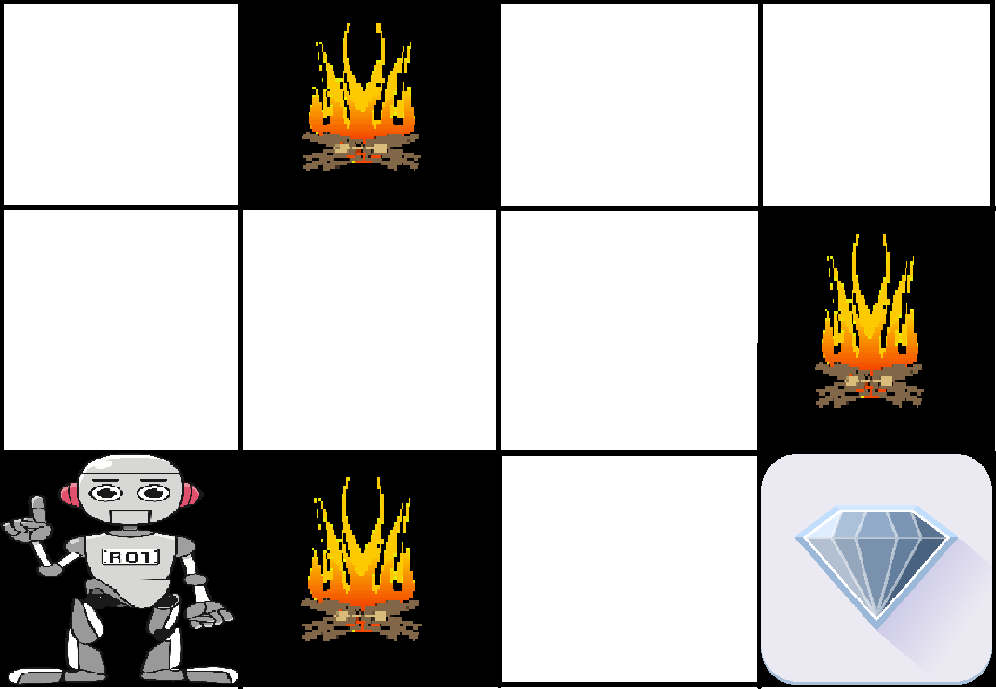
\includegraphics[width=\linewidth]{RL_robot.png}};
        \end{tikzpicture}
    \caption{An agent has to reach a reward without burning}
    \end{figure}
    \column{.3\textwidth}
    \begin{itemize}
        \item policy learning
        \item value learning
    \end{itemize}
    \end{columns}
\end{frame}
\subsection{Basics}

\subsection{Application to TP}
\begin{frame}
    \frametitle{Application to TP}
    RL to TP mapping:
    \begin{columns}
    \column{.7\textwidth}
    \begin{itemize}
        \item agent $\leftrightarrow$ TP
        \item environment $\leftrightarrow$ search tree
        \item actions $\leftrightarrow$ extending search tree
        \item reward $\leftrightarrow$ finding a closed tableau
    \end{itemize}
    \column{.3\textwidth}
    \begin{figure}
    \centering
    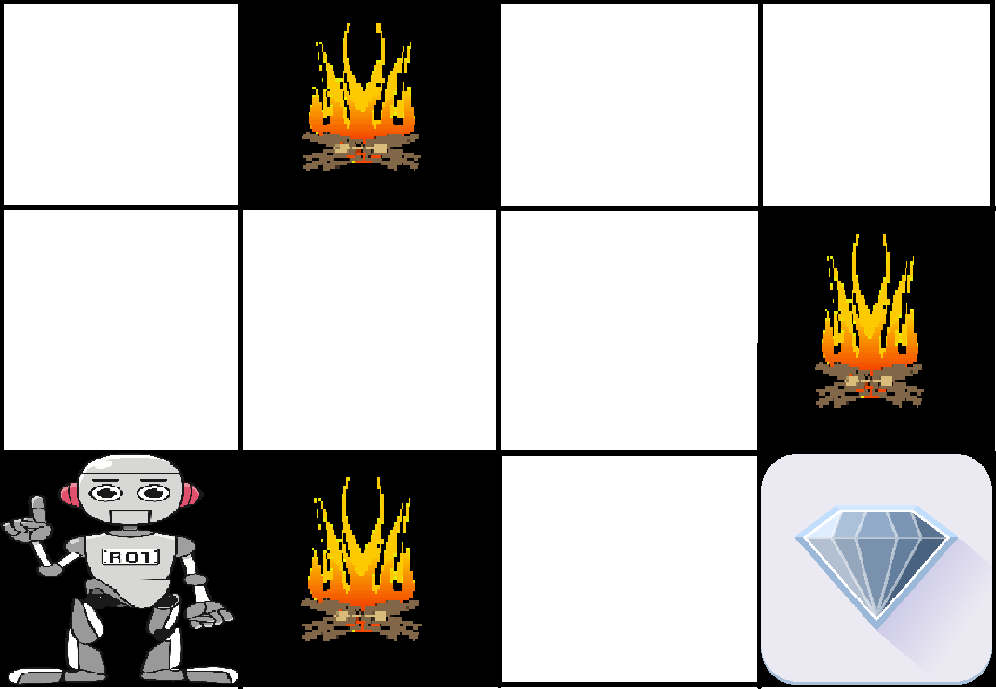
\includegraphics[width=\textwidth]{RL_robot.png}
    \end{figure}
    \end{columns}
\end{frame}

\begin{frame}
    \frametitle{Application to TP -- the UCT formula}
    Tree search with RL -- use the UCT formula!\\
    For each node $i$:
    \begin{columns}
        \centering
    \column{.69\textwidth}
    \begin{equation*}
        f_i=\frac{w_i}{n_i}+c\cdot p_i \cdot \sqrt{\frac{\ln N_i}{n_i}}
    \end{equation*}
    \column{.40\textwidth}
    \begin{itemize}
        \small
        \item[$w_i$:] \textbf{total reward}
        \item[$n_i$:] number node of visits
        \item[$c$:] hyperparameter
        \item[$p_i$:] \textbf{prior probability}
        \item[$N_i$:] total parent visits
    \end{itemize}
    \end{columns}

    On every step, take the node with highest $f_i$.
    % Without any learning, all prior probabilities are equal and the values are
    % determined by the number of open goals.
\end{frame}

\begin{frame}
    \frametitle{Application to TP -- Extracting features (Literals)}
    \begin{columns}
    \column{.7\textwidth}
    \begin{itemize}
        \item For each Literal $L$, e.g. $f(X, Y) = g(sk_1, sk_2(X))$
        \item Build it's feature tree
        \item Count term walks of length 3
        \item E.g. for L we get {\small$\{(\oplus, =, f): 1, (=, f, \oast):2, ...\}$}
    \end{itemize}
    \column{.2\textwidth}
    \begin{figure}
    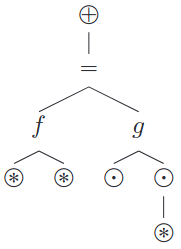
\includegraphics[width=\textwidth]{AST.png}
    \caption{Feature Tree for $L$}
    \end{figure}
    \end{columns}
    \let\thefootnote\relax\footnotetext{Example and picture from \cite{Enigma}}

    % \textbf{Step 2:} Getting the data:
    %     \begin{itemize}
    %         \item Run many Monte-Carlo proof searches
    %         \item 
    %     \end{itemize}
\end{frame}

\begin{frame}
    \frametitle{Application to TP -- Extracting features}
    \begin{itemize}
        \item Features for a \emph{clause} -- union of features for literals
        \pause
        \item Feature vector for a \emph{state}:
            \begin{itemize}
                \item Features of clauses and goals
                \item additional metadata -- No. of open goals, depth of node, etc.
            \end{itemize}
        \pause
        \item Features for an \emph{action} contains:
            \begin{itemize}
                \item features of the clause used
                \item features of literal used
            \end{itemize}
    \end{itemize}
\end{frame}

\begin{frame}
    \frametitle{Application to TP -- Learning the parameters}
    \begin{itemize}
        \item Start with unrestricted Monte-Carlo TP runs:
        \begin{equation*}
            f_i=\frac{w_i}{n_i}+c\cdot p_i \cdot \sqrt{\frac{\ln N_i}{n_i}}
        \end{equation*}
        \item<2-> Learn action $a$ relevance given $f_s$ and $f_a$
            \begin{itemize}
                \item $r_a=\dfrac{overal\ frequency\ of\ a}{action\ frequency\ at\ node}$ 
                \item $r_a \in (0, \infty)$
                \item $p_i=softmax(r_a, R)$ 
            \end{itemize}
        \item<3-> Associate node state feature with value
            \begin{itemize}
                \item 0 if node not a proof
                \item $0.99^{proof\ depth}$ otherwise
            \end{itemize}
        \item<4-> Apply regression on the logits to learn prior probability and value
        \item<4-> \textbf{Deduce}, \textbf{Learn} from it, and \textbf{Loop}
    \end{itemize}
\end{frame}

\subsection{Results}

\begin{frame}
\frametitle{Results}
\begin{itemize}
    \item 90\%-10\% split on the Mizar Mathematical Library \citep{MML} .
    \item training set is $\approx 30K$ problems, testing -- $\approx 3.2K$
\end{itemize}
\begin{table}
\begin{tabular}{l l l l l}
\toprule
Iteration & 1 & 2 & 5 & 8 \\
Training Proved & 12325 & 13749 & 14403 & 14498\\
Testing Proved & 1354 &  1519 & 1624 & 1591\\
\bottomrule
\end{tabular}
\caption{Proved problems per iterations of learning}
\end{table}

\pause
\begin{table}
\begin{tabular}{l l l}
\toprule
\textbf{Methodology} & \textbf{Proved} & \textbf{IPS} \\
\midrule
Heuristics tableaux & 1143 & 64K \\
RL tableaux & 1624 & 16K \\

\bottomrule
\end{tabular}
\caption{Using RL gives 40\% more proves but slows down the inference speed}
\end{table}
\end{frame}

\section{Summary}

\begin{frame}
\frametitle{Summary}
\begin{itemize}
    \item ML (RL) application on Theorem Provers
    \item Helps `discover' new proofs!
    \item ... but slows down inference speed
\end{itemize}

\end{frame}
\begin{frame}
\Huge
\centering
Questions?
\end{frame}
%% TODO DELETE BELOW
%\begin{frame}
%\frametitle{Paragraphs of Text}
%\end{frame}

%%------------------------------------------------


%\begin{frame}
%\frametitle{Blocks of Highlighted Text}
%\begin{block}{Block 1}
%Lorem ipsum dolor sit amet, consectetur adipiscing elit. Integer lectus nisl, ultricies in feugiat rutrum, porttitor sit amet augue. Aliquam ut tortor mauris. Sed volutpat ante purus, quis accumsan dolor.
%\end{block}

%\begin{block}{Block 2}
%Pellentesque sed tellus purus. Class aptent taciti sociosqu ad litora torquent per conubia nostra, per inceptos himenaeos. Vestibulum quis magna at risus dictum tempor eu vitae velit.
%\end{block}

%\begin{block}{Block 3}
%Suspendisse tincidunt sagittis gravida. Curabitur condimentum, enim sed venenatis rutrum, ipsum neque consectetur orci, sed blandit justo nisi ac lacus.
%\end{block}
%\end{frame}

%%------------------------------------------------

%\begin{frame}
%\frametitle{Multiple Columns}
%\begin{columns}[c] % The "c" option specifies centered vertical alignment while the "t" option is used for top vertical alignment

%\column{.45\textwidth} % Left column and width
%\textbf{Heading}
%\begin{enumerate}
%\item Statement
%\item Explanation
%\item Example
%\end{enumerate}

%\column{.5\textwidth} % Right column and width
%Lorem ipsum dolor sit amet, consectetur adipiscing elit. Integer lectus nisl, ultricies in feugiat rutrum, porttitor sit amet augue. Aliquam ut tortor mauris. Sed volutpat ante purus, quis accumsan dolor.

%\end{columns}
%\end{frame}

%%------------------------------------------------
%\section{Second Section}
%%------------------------------------------------

%\begin{frame}
%\frametitle{Table}

%\begin{table}
%\begin{tabular}{l l l}
%\toprule
%\textbf{Treatments} & \textbf{Response 1} & \textbf{Response 2}\\
%\midrule
%Treatment 1 & 0.0003262 & 0.562 \\
%Treatment 2 & 0.0015681 & 0.910 \\
%Treatment 3 & 0.0009271 & 0.296 \\
%\bottomrule
%\end{tabular}
%\caption{Table caption}
%\end{table}

%\end{frame}

%%------------------------------------------------

%\begin{frame}
%\frametitle{Theorem}
%\begin{theorem}[Mass--energy equivalence]
%$E = mc^2$
%\end{theorem}
%\end{frame}

%%------------------------------------------------

%\begin{frame}[fragile] % Need to use the fragile option when verbatim is used in the slide
%\frametitle{Verbatim}
%\begin{example}[Theorem Slide Code]
%\end{example}
%\end{frame}

%%------------------------------------------------

%\begin{frame}
%\frametitle{Figure}
%Uncomment the code on this slide to include your own image from the same directory as the template .TeX file.
%%\begin{figure}
%%\includegraphics[width=0.8\linewidth]{test}
%%\end{figure}
%\end{frame}

%%------------------------------------------------

%\begin{frame}[fragile] % Need to use the fragile option when verbatim is used in the slide
%\frametitle{Citation}
%\cite{MaLARea}
%% An example of the \verb|\cite| command to cite within the presentation:\\~

%% This statement requires citation \cite{p1}.
%\end{frame}

%%------------------------------------------------

%%------------------------------------------------

\begin{frame}{Bibliography}
\bibliographystyle{apalike}
\bibliography{../refs.bib}
\end{frame}

%----------------------------------------------------------------------------------------

\end{document} 
